\section{Cone Theorem}


\subsection{Preliminary}

    \begin{theorem}[{Iitaka fibration, semiample case, ref. \cite[Theorem 2.1.27]{Laz04a}}]\label{thm: Iitaka fibration in semiample case}
        Let \(X\) be a projective variety and \(\calL\) an semiample line bundle on \(X\).
        Then there exists a fibration \(\varphi: X \to Y\) of projective varieties 
        such that for any \(m\gg 0\) with \(\calL^m\) base point free, we have that the morphism \(\varphi_{\calL^m}\) induced by \(\calL^m\) is isomorphic to \(\varphi\).
        Such a fibration is called the \emph{Iitaka fibration} associated to \(\calL\).
    \end{theorem}

    \begin{theorem}[{Rigidity Lemma, ref. \cite[Lemma 1.15]{Deb01}}]\label{thm: Rigidity Lemma}
        Let \(\pi_i: X \to Y_i\) be proper morphisms of varieties over a field \(\kk\) for \(i=1,2\).
        Suppose that \(\pi_1\) is a fibration and \(\pi_2\) contracts \(\pi_1^{-1}(y_0)\).
        Then there exists a rational map \(\varphi: Y_1 \ratmap Y_2\) such that \(\pi_2 \circ \varphi = \pi_1\) and \(\varphi\) is well-defined near \(Y_1 \setminus \{y_0\}\). 
    \end{theorem}

    \begin{theorem}\label{thm:convex_separation_theorem}
        Let \(A,B \subset \bbR^n\) be disjoint convex sets.
        Then there exists a linear functional \(f: \bbR^n \to \bbR\) such that \(f|_A \leq c\) and \(f|_B \geq c\) for some \(c \in \bbR\).
    \end{theorem}

    % \begin{theorem}[{Upper semicontinuity of cohomology, ref. \cite[Chapter III, Theorem 12.8]{Har77}}]\label{thm: upper semicontinuity of cohomology}
    %     Let \(f:X \to Y\) be a projective morphism of noetherian schemes and \(\calf\) a coherent sheaf on \(X\) flat over \(Y\).
    %     Then the function \(y \mapsto h^i(y,\calf)\) is upper semicontinuous on \(Y\) for every \(i\).   
    % \end{theorem}

    % \begin{theorem}[{Grauert's Theorem, ref. \cite[Chapter III, Corollary 12.9]{Har77}}]\label{thm: Grauert's Theorem}
    %     Let \(f:X \to Y\) be a projective morphism of noetherian schemes and \(\calf\) a coherent sheaf on \(X\) flat over \(Y\).
    %     Suppose that \(Y\) is integral and \(h^i(y,\calf)\) is constant on \(Y\) for some \(i\).
    %     Then \(R^if_*\calf\) is locally free sheaf on \(Y\) and the natural map \(R^if_*\calf \ten \rkk(y) \to H^i(X_y,\calf_y)\) is an isomorphism for every \(y \in Y\).
    % \end{theorem}

    \begin{proposition}\label{prop:general_rational_curve_on_klt_variety_with_negative_intersection}
        Let \(X\) be a normal projective variety of dimension \(n\) and \(H\) an ample divisor on \(X\).
        Suppose that \(K_X\cdot H^{n-1} < 0\).
        Then for a general point \(x\in X\), there exists a rational curve \(\Gamma\) passing through \(x\) such that
        \[ 0 < H \cdot \Gamma \leq - 2n \cdot \frac{H^n}{K_X \cdot H^{n-1}}. \]
    \end{proposition}
    \begin{proof}[Schetch of proof]
        % Choose a curve \(C = H^{n-1}\) such that \(X\) is smooth near \(C\).
        Take a resolution \(f:Y \to X\), then \(f^*H\) is nef on \(Y\) and \(K_Y\cdot f^*H^{n-1} < 0\) since \(E \cdot f^*H^{n-1} = 0\).
        Choose an ample divisor \(H_Y\) on \(Y\) closed enough to \(f^*H\) such that \(K_Y \cdot H_Y^{n-1} < 0\).
        By \cite[Theorem 5]{MM86} and take limit for \(H_Y\).
    \end{proof}

    \begin{lemma}[{ref. \cite[Lemma]{Kaw91}}]\label{lem:the_pair_controls_the_exceptional_locus}
        Let \((X,B)\) be a projective klt pair and \(f:X \to Y\) a birational projective morphism.
        Let \(E\) be an irreducible component of dimension \(d\) of the exceptional locus of \(f\) and \(\nu:E^\nu \to X\) the normalization of \(E\).
        Suppose that \(f(E)\) is a point.
        Then for any ample divisor \(H\) on \(X\), we have
        \[ K_{E^\nu}\cdot \nu^*H^{d-1} \leq K_{(X,B)}|_{E^\nu}\cdot \nu^*H^{d-1}. \]
    \end{lemma}

    % \begin{lemma}\label{lem:higher_direct_image_of_exceptional_divisor}
    %     Let \(f:Y \to X\) be a birational morphism of projective varieties with \(Y\) smooth and \(X\) has only rational singularities.
    %     Let \(E\) be an effective exceptional divisor on \(Y\) and \(D\) a divisor on \(X\).
    %     Then we have
    %     \[ f_*(\calo_Y(f^*D + E)) \cong \calo_X(D), \quad R^if_*(\calo_Y(f^*D + E)) = 0,\quad \forall i > 0. \]
    % \end{lemma}
    % \begin{proof}
    %     \Yang{I am unable to proof this lemma.}
    % \end{proof}

\subsection{Non-vanishing Theorem}

    \begin{theorem}[Non-vanishing Theorem]\label{thm: non-vanishing theorem}
        Let \((X,B)\) be a projective klt pair and \(D\) a Cartier divisor on \(X\).
        Suppose that \(D\) is nef and \(aD-K_{(X,B)}\) is nef and big for some \(a > 0\).
        Then for \(m \gg 0\), we have 
        \[ H^0(X,mD) \neq 0. \]
    \end{theorem}
    \begin{proof}
        \Yang{To be completed.}
    \end{proof}

\subsection{Base Point Free Theorem}

    \begin{theorem}[Base Point Free Theorem]\label{thm: base point free theorem}
        Let \((X,B)\) be a projective klt pair and \(D\) a Cartier divisor on \(X\).
        Suppose that \(D\) is nef and \(aD-K_{(X,B)}\) is nef and big for some \(a > 0\).
        Then for \(m \gg 0\), \(mD\) is base point free.
    \end{theorem}
    \begin{proof}
        \Yang{To be completed.}
    \end{proof}

    \begin{remark}\label{rmk:statement_in_BPF_theorem_stronger_than_semiample}
        In general, we say that a Cartier divisor \(D\) is \emph{semiample} if there exists a positive integer \(m\) such that \(mD\) is base point free.
        The statement in Base Point Free Theorem (\cref{thm: base point free theorem}) is strictly stronger than the semiample condition.
        For example, let \(\calL\) be a torsion line bundle, then \(\calL\) is semiample, but there exists no positive integer \(M\) such that \(m\calL\) is base point free for all \(m>M\).
    \end{remark}

\subsection{Rationality Theorem}

    

    % \begin{lemma}\label{lem:polynomial_vanishes_along_strips}
    %     Let \(P(x,y) \neq 0\in \bbQ[x,y]\) with \(\deg P \leq n\).
    %     Then for every \(r,\varepsilon > 0\) with \(n+1 \leq v(r)\varepsilon\) and for all \(M>0\), \(P\) is not identically zero on the set 
    %     \[ \Lambda_{r,\varepsilon} \coloneqq \{(p,q) \in \bbZ^2 : p,q>M, 0\leq pr-q \leq \varepsilon\}.\]
    %     \Yang{Need to modify}
    % \end{lemma}
    % \begin{proof}
    %     If \(v(r)=v < \infty\), then for all \(m > 0\), there is a line \(L \)

    %     \Yang{To be completed.}
    % \end{proof}

    \begin{lemma}[{ref. \cite[Theorem 1.36]{KM98}}]\label{lem:Hilbert_polynomial}
        Let \(X\) be a proper variety of dimension \(n\) and \(D_1,\ldots,D_m\) Cartier divisors on \(X\).
        Then the Euler characteristic \(\chi(n_1D_1,\ldots,n_mD_m)\) is a polynomial in \((n_1,\cdots,n_m)\) of degree at most \(n\).
    \end{lemma}

    \begin{theorem}[Rationality Theorem]\label{thm: rationality theorem}
        Let \((X,B)\) be a projective klt pair, \(a = a(X) \in \bbZ\) with \(aK_{(X,B)}\) Cartier and \(H\) an ample divisor on \(X\).
        Let 
        \[ t \coloneqq \inf \{s \geq 0: K_{(X,B)} + sH \text{ is nef}\} \]
        be the nef threshold of \((X,B)\) with respect to \(H\).
        Then \(t = v/u \in \bbQ\) and 
        \[ 0 \leq v \leq a(X)\cdot (\dim X + 1). \]
    \end{theorem}
    \begin{proof}
        For every \(r \in \bbR_{> 0}\), let 
        \[ v(r) \coloneqq \begin{cases}
            v, & \text{if } r = \frac{v}{u} \in \bbQ \text{ in lowest term; } \\
            \infty, & \text{if } r \in \bbR\setminus \bbQ.
        \end{cases} \]
        We need to show that \(v(t) \leq a(\dim X + 1)\).
        For every \((p,q) \in \bbZ_{>0}^2\), set \(D(p,q) \coloneqq paK_{(X,B)} + qH\).
        If \((p,q)\in \bbZ^2_{>0}\) with \(0< atp-q < t\), then we have \(D(p,q)\) is not nef and \(D(p,q) - K_{(X,B)}\) is ample.

        \begin{step}\label{step_in_thm:rationality_theorem:polynomial_non-vanishing_on_strips}
            We show that a polynomial \(P(x,y) \neq 0 \in \bbQ[x,y]\) of degree at most \(n\) is not identically zero on the set
            \[  \{(p,q) \in \bbZ^2 : p,q>M, 0< atp-q < t\varepsilon\}, \quad \forall M > 0, \] 
            if \(v(t)\varepsilon > a(n+1)\). 
        \end{step}
        If \(v(t) = \infty\), for any \(n\), we show that we can find infinitely many lines \(L\) such that \(\#L\cap \Lambda \geq n+1\).
        If so, \(\Lambda\) is Zariski dense in \(\bbQ^2\).
        Since \(1/at\in \bbR\setminus \bbQ\), there exist \(p_0,q_0>M\) such that 
        \[ 0 < \frac{p_0}{q_0} - \frac{1}{at} < \frac{\varepsilon}{(n+1)a} \cdot \frac{1}{q_0}, \text{ i.e. } 0<atp_0 - q_0 < \frac{\varepsilon t}{n+1}. \]
        Then \((ip_0,iq_0) \in \Lambda \cap \{p_0y=q_0x\}\) for \(i = 1,\cdots,n+1\).
        Since \(M\) is arbitrary, there are infinitely many such lines \(L\).
        
        Suppose \(v(t) = v < \infty\) and \(t = v/u\).
        Then the inequality is equivalent to \(0 < aup - vq < \varepsilon v\).
        Note that \(\gcd(au,v) | a\), then \(aup - vq = a i\) has integer solutions for \(i = 1,\cdots,n+1\).
        Since \(v(t)\varepsilon > a(n+1)\), there are at least \(n+1\) lines which intersect \(\Lambda\) in infinitely many points.
        This enforce any polynomial which vanishes on \(\Lambda\) has degree at least \(n+1\).
        % \Yang{To be completed.}

        \begin{step}
            There exists an index set \(\Lambda \subset \bbZ^2\) such that \(\Lambda\) contains all sufficiently large \((p,q)\) with \(0 \leq at p - q \leq t\) and 
            \[ Z \coloneqq \Bs |D(p,q)| = \Bs |D(p',q')| \neq \emptyset, \quad \forall (p,q), (p',q') \in \Lambda. \]
        \end{step}
        For every \((p,q) \in \bbZ^2_{>0}\) with \(0 < atp-q < t\), there exists \(M > 0\) such that 
        \[D(\alpha,\beta) = \alpha a K_{(X,B)} + \beta H\]
        is base point free for all \(\alpha = 0,\cdots,p\) and \(\beta > M\).
        Choose \(M'\) large enough such that for all \((p',q') \in \bbZ^2_{>0}\) with \(p',q' > M'\) and \(0 < atp'-q' < t\), write
        \[ p' = lp + p_0, \quad q' = lq + q_0 \]
        for some \(l \in \bbZ_{\geq 0}\) and \(0 \leq p_0 < p\),
        we have \(q_0 > M\).
        The existence of such \(M'\) follows from the estimate
        \[ q_0 = q' - lq = q' - \frac{p'-p_0}{p}q > q' - (p'-p_0)(at-\delta) > p'\delta, \]
        where \(\delta > 0\) is a small enough number such that \(at - \delta > q/p\).
        \[ 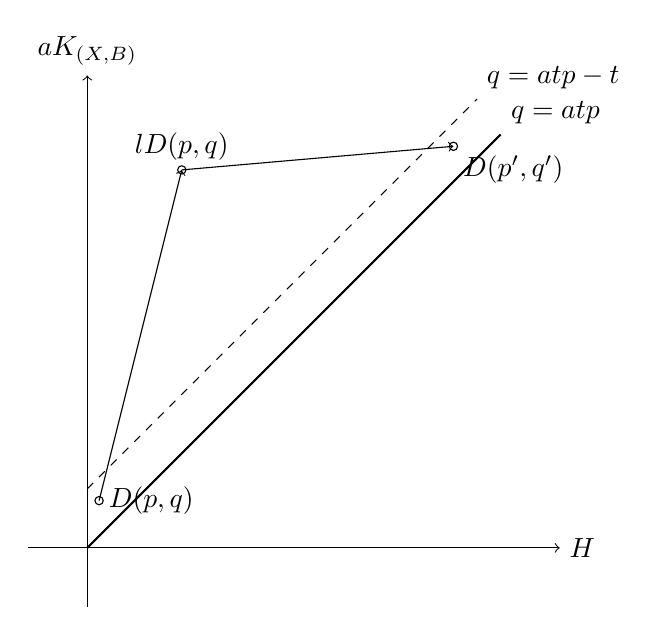
\begin{tikzpicture}[scale=1.5]
            \draw[->] (-0.5,0) -- (4,0) node[right] {\(H\)};
            \draw[->] (0,-0.5) -- (0,4) node[above] {\(aK_{(X,B)}\)};
            \draw[thick] (0,0) -- (3.5,3.5) node[above right] {\(q = atp\)};
            \draw[dashed] (0,0.5) -- (3.3,3.8) node[above right] {\(q = atp - t\)};
            \draw (0.1,0.4) circle (1pt) node[right] {\(D(p,q)\)};
            \draw (0.8,3.2) circle (1pt) node[above] {\(lD(p,q)\)};
            \draw[->] (0.1,0.4) -- (0.8,3.2);
            \draw (3.1,3.4) circle (1pt) node[below right] {\(D(p',q')\)};
            \draw[->] (0.8,3.2) -- (3.1,3.4);
        \end{tikzpicture} \]
        Then \(D(p',q') - lD(p,q) = D(p_0,q_0)\) is base point free.
        It follows that \(\Bs |D(p',q')| \subseteq \Bs |D(p,q)|\).
        By noetherian induction, there exists an index set \(\Lambda\) such that \(\Bs |D(p,q)| = Z\) for all \((p,q) \in \Lambda\).
        % \Yang{To be completed.}

        \begin{step}\label{step_in_thm:rationality_theorem:non-vanishing_on_strips}
            Suppose the contradiction that \(v(t) > a(\dim X + 1)\).
            Then we show that \(H^0(X,D(p,q)) \neq 0\) for all \((p,q) \in \Lambda\).
            This is an analogue of Non-vanishing Theorem in the proof of Base Point Free Theorem (\cref{thm: base point free theorem}).
        \end{step}
        Let \(P(x,y)\coloneqq \chi(D(x,y))\) be the Hilbert polynomial of \(D(x,y)\).
        Note that \(P(0,n) = \chi(nH) \neq 0\) since \(H\) is ample.
        Then \(P(x,y) \neq 0\) and \(\deg P \leq \dim X\).
        By \cref{step_in_thm:rationality_theorem:polynomial_non-vanishing_on_strips}, \(P\) is not identically zero on \(\Lambda\).
        Note that \(D(p,q) - K_{(X,B)}\) is ample for all \((p,q) \in \Lambda\), then \(h^i(X,D(p,q)) = 0\) for all \(i > 0\) by Kawamata-Viehweg vanishing theorem (\cref{thm: Kawamata-Viehweg Vanishing Theorem for klt pair}).
        Then 
        \[ P(p,q) = \chi(D(p,q)) = h^0(X,D(p,q)) \neq 0 \]
        for some \((p,q) \in \Lambda\).
        This is equivalent to that \(Z \neq X\) and hence \(H^0(X,D(p,q)) \neq 0\) for all \((p,q) \in \Lambda\).

        % \Yang{To be completed.}

        \begin{step}
            We follow the same line of the proof of Base Point Free Theorem (\cref{thm: base point free theorem}) to show that there is a section which does not vanish on \(Z\).
        \end{step}
        Fix \((p,q) \in \Lambda\).
        If \(v(t) < \infty\), we assume that \(t=v/u\) and \(atp-q = a(n+1)/u\).
        Let \(f:Y \to X\) be a resolution such that 
        \begin{enumerate}
            \item \(K_{Y,B_Y} = f^*K_{(X,B)} + E_Y\) for some effective exceptional divisor \(E_Y\), and \(Y,B_Y\) is a klt pair;
            \item \(f^*|D(p,q)| = |L| + F\) for some effective divisor \(F\) and a base point free divisor \(L\), and \(f(\Supp F) = Z\);
            \item \(f^*D(p,q) - f^*K_{(X,B)} - E_0\) is ample for some effective \(\bbQ\)-divisor \(E_0 \in (0,1)\), and coefficients of \(E_0\) are sufficiently small;
            \item \(B_Y + E_Y + F + E_0\) has snc support.
        \end{enumerate}
        \Yang{Such resolution exists by \cite{KM98}.}

        Let \(c := \inf\{ \lfloor B_Y + E_0 + t F \rfloor \neq 0\}\).
        Adjust the coefficients of \(E_0\) slightly such that \(\lfloor B_Y + E_0 + c F \rfloor = F_0\) for unique prime divisor \(F_0\) with \(F_0 \subset \Supp F\).
        Set \(\Delta_Y \coloneqq B_Y + c F + E_0 - F_0\).
        Then \((Y,\Delta_Y)\) is a klt pair.

        Let 
        \begin{align*}
            N(p',q') &\coloneqq f^*D(p',q') + E_Y - F_0 - K_{(Y,\Delta_Y)}  \\
                & = \Big(f^*D(p',q') - (1+c)f^*D(p,q)\Big) + \Big(f^*D(p,q) - f^*K_{(X,B)} - E_0\Big) + c \Big(f^*D(p,q) - F\Big).
        \end{align*} 
        Note that on 
        \[ \Lambda_0 := \{(p',q') \in \Lambda: 0< atp' - q' < atp - q,\  p',q'>(1+c)\max\{p,q\}\}, \]
        the divisor \(f^*D(p',q') - (1+c)f^*D(p,q) = f^*D(p'-(1+c)p,q'-(1+c)q)\) is ample, and hence \(N(p',q')\) is ample.

        By the exact sequence 
        \[ 0 \to \calo_Y(f^*D(p',q')+E_Y-F_0) \to \calo_Y(f^*D(p',q')+E_Y) \to \calo_{F_0}((f^*D(p',q')+E_Y)|_{F_0}) \to 0 \]
        and Kawamata-Viehweg Vanishing Theorem (\cref{thm: Kawamata-Viehweg Vanishing Theorem for klt pair}), we get a surjective map
        \[ H^0(Y,f^*D(p',q')+E_Y) \surjmap H^0(F_0,(f^*D(p',q')+E_Y)|_{F_0}). \]
        On \(F_0\), consider the polynomial \(\chi((f^*D(p',q')+E_Y)|_{F_0})\).
        Note that \(\dim F_0 = n-1\) and by the construction of \((p,q),\Lambda_0\), 
        similar to \cref{step_in_thm:rationality_theorem:non-vanishing_on_strips}, 
        we can show that \(\chi((f^*D(p',q')+E_Y)|_{F_0})\) is not identically zero on \(\Lambda_0\).
        By adjunction, we have \((f^*D(p',q')+E_Y)|_{F_0} = N(p',q')|_{F_0} + K_{(F_0,\Delta_Y|_{F_0})}\) with \(N(p',q')|_{F_0}\) ample and \((F_0,\Delta_Y|_{F_0})\) klt.
        Hence we can apply Kawamata-Viehweg Vanishing Theorem (\cref{thm: Kawamata-Viehweg Vanishing Theorem for klt pair}) to get
        \[ h^0(F_0,(f^*D(p',q')+E_Y)|_{F_0}) = \chi(F_0,(D(p',q')+E_Y)|_{F_0}) \neq 0.\]
        This combining with the surjective map contradict to the assumption that \(f(F_0) \subset Z = \Bs |D(p',q')|\).
    \end{proof}


\subsection{Cone Theorem and Contraction Theorem}

    \begin{theorem}[Cone Theorem]\label{thm: cone theorem}
        Let \((X,B)\) be a projective klt pair.
        Then there exist countably many curves \(C_i \subset X\) 
        % with 
        % \[ 0 < -K_{(X,B)} \cdot C_i \leq 2 \dim X \]
        such that 
        \begin{enumerate}
            \item we have a decomposition of cones
            \[ \Psef_1(X) = \Psef_1(X)_{K_{(X,B)} \geq 0} + \sum \bbR_{\geq 0}[C_i]; \]
            \item and for any \(\varepsilon > 0\) and an ample divisor \(H\) on \(X\), we have 
            \[ \Psef_1(X) = \Psef_1(X)_{K_{(X,B)}+\varepsilon H \geq 0} + \sum_{\text{finite}} \bbR_{\geq 0}[C_i]. \]
        \end{enumerate}
    \end{theorem}
    \begin{proof}
        Let \(F_D \coloneqq \Psef_1(X) \cap D^\perp\) for a nef divisor \(D\) on \(X\).
        If \(\dim F_D = 1\), we also write \(R_D \coloneqq F_D\).
        Let \(H_1,\cdots,H_{\rho-1}\) be ample divisors on \(X\) such that they together with \(K_{(X,B)}\) form a basis of \(N^1(X)_\bbQ\).
        Fix a norm \(\|\cdot\|\) on \(N_1(X)_\bbR\) and let \(S^{\rho-1} \coloneqq S(N_1(X)_\bbR)\) be the unit sphere in \(N_1(X)_\bbR\).
        
        \begin{step}\label{step_in_thm:cone_theorem:negative_extremal_faces_will_be_stable}
            There exists an integer \(N\) such that for every \(K_{(X,B)}\)-negative extremal face \(F_D\) and for every ample divisor \(H\), 
            there exists \(n_0, r \in \bbZ_{>0}\) such that for all \(n>n_0\), \(\{0\} \neq F_{nD+rK_{(X,B)}+N H} \subset F_D\). 
        \end{step}
        Let \(N \coloneqq (a(X)(\dim X + 1))!\), where \(a(X)\) is the number in \cref{thm: rationality theorem}.
        For every \(n\), \(nD+H\) is an ample divisor and by \cref{thm: rationality theorem}, the nef threshold of \(K_{(X,B)}\) with respect to \(nD+H\) is of form
        \[ \inf \{s \geq 0: K_{(X,B)} + s(nD+H) \text{ is nef}\} = \frac{N}{r_n}, \quad r_n \in \bbZ_{\geq 0}. \]
        Since \(K_{(X,B)} + (N/r_n)((n+1)D+H)\) is nef, we have \(r_{n} \leq r_{n+1}\).
        On the other hand, let \(\xi \in F_{D}\setminus \{0\}\). 
        Then \(\xi \cdot (K_{(X,B)} + (N/r_n)(nD+H)) \geq 0\) implies that
        \[ r_n \leq - N \cdot \frac{K_{(X,B)}\cdot \xi}{H \cdot \xi}. \]
        Hence \(r_n \to r \in \bbZ_{\geq 0}\).
        It follows that \(rK_{(X,B)}+nND+NH\) is a nef but not ample divisor for all \(n \gg 0\).
        Note that for every nef divisors \(N_1,N_2\), we have \(F_{N_1+N_2} = F_{N_1} \cap F_{N_2}\).
        Then for all \(n \gg 0\), there exists \(m\) large enough such that
        \[ \{0\} \neq F_{rK_{(X,B)}+mND+N H} \subset F_{rK_{(X,B)}+nD+NH} \subset F_D. \]

        \begin{step}\label{step_in_thm:cone_theorem:nagetive_extremal_rays_form_a_lattice}
            Let \(\Phi: N_1(X)_{K_{(X,B)}<0} \to \bbR^{\rho-1}\) be the map defined by 
            \[ \alpha \mapsto \left( \frac{H_1 \cdot \alpha}{K_{(X,B)}\cdot \alpha},\ldots, \frac{H_{\rho-1} \cdot \alpha}{K_{(X,B)}\cdot \alpha}\right). \]
            We show that the image of \(R_D\) under \(\Phi\) lies in a \(\bbZ\)-lattice in \(\bbR^{\rho-1}\).
        \end{step}
        Suppose \(R = \bbR_{\geq 0}\xi\) for a class \(\xi\).
        By \cref{step_in_thm:cone_theorem:negative_extremal_faces_will_be_stable}, we have \(R_{nD+rK_{(X,B)}+N H_i} = R_{D}\) for some integers \(n,r\).
        Then \( \xi \cdot (nD+rK_{(X,B)}+N H_i) = 0 \) implies that
        \[ \frac{H_i \cdot \xi}{K_{(X,B)}\cdot \xi} = \frac{-r}{N} \in \frac{1}{N}\bbZ. \]
        It follows that the image of \(R_D\) under \(\Phi\) lies in \(\frac{1}{N} \bbZ^{\rho-1}\).

        \begin{step}\label{step_in_thm:cone_theorem:negative_extremal_rays_are_rational}
            We show that every \(K_{(X,B)}\)-negative extremal ray of \(\Psef_1(X)\) is of the form \(R_D\) for some nef divisor \(D\) on \(X\).
        \end{step}
        Let \(R = \bbR_{\geq 0}\xi\) be a \(K_{(X,B)}\)-negative exposed ray.
        % \Yang{Then \(R\) is of form \(D^\perp \cap \Psef_1(X)\) for some nef \(\bbR\)-divisor \(D\) on \(X\) by \cref{thm:convex_separation_theorem}.}
        % \Yang{This is wrong, we need the Straszewicz theorem to get an exposed ray.}
        Then \(R\) is of form \(D^\perp \cap \Psef_1(X)\) for some nef \(\bbR\)-divisor \(D\) on \(X\).
        We need to show that \(D\) can be choose as a nef \(\bbQ\)-divisor.
        There is a sequence of nef but not ample \(\bbQ\)-divisors \(D_m\) such that \(D_m \to D\) as \(m \to \infty\).
        We adjust \(D_m\) such that \(\dim F_{D_m} = 1\) for all \(n\).

        By re-choosing \(H_i\), we can assume that \(D = a_1H_1 + \cdots + a_{\rho-1}H_{\rho-1} + a_\rho K_{(X,B)}\) for \(a_i > 0\) since \(aD-K\) is ample for \(a \gg 0\).
        After truncation, we can assume that so is \(D_m\).
        Then \(F_{D_m}\) is \(K_{(X,B)}\)-negative.
        Note that \(F_{nD_m+r_iK_{(X,B)} + N H_i} \subset F_{D_m}\) for some \(r_i>0\) and \(n\gg 0\) by \cref{step_in_thm:cone_theorem:negative_extremal_faces_will_be_stable}.
        If \(\dim F_{D_m} > 1\), then not all \(H_i|_{F_{D_m}}\) are proportional to \(K_{(X,B)}|_{D_m}\).
        We can assume that\(r_1K_{(X,B)}+N H_1\) is not identically zero on \(F_{D_m}\).
        Then we can choose \(n\) large enough such that \(\|r_1K_{(X,B)}+N H_1\|/n < 1/m\).
        Replace \(D_m\) by \(D_m + (r_1K_{(X,B)}+N H_1)/n\).
        Inductively we construct \(D_m\) nef \(\bbQ\)-divisor with \(D_m \to D\) and \(\dim F_{D_m} = 1\).
        
        Let \(R_{D_m} = \bbR_{\geq 0} \xi_m\).
        Suppose that \(\|\xi_m\|=\|\xi\| = 1\).
        By passing to a subsequence, we can assume that \(\xi_m\) converges.
        Then \(\xi_m \to \xi\) since \(\lim D_m \cdot \xi_m = D \cdot \lim \xi_m = 0\).
        However, \(\Phi\) is well-defined at \(\xi\) and the image of \(\xi_m\) under \(\Phi\) is discrete.
        Hence \(\xi=\xi_m\) for all \(m\) large enough.
        It follows that \(R = R_{D_m}\) for a nef \(\bbQ\)-divisor \(D_m\).

        By \cref{step_in_thm:cone_theorem:nagetive_extremal_rays_form_a_lattice}, the \(K_{(X,B)}\)-negative extremal rays form a discrete set in \(\{\alpha \in \Psef_1(X): K_{(X,B)}\cdot \alpha < 0\}\).
        Hence every \(K_{(X,B)}\)-negative extremal ray is an exposed ray by Straszewicz's Theorem.

        % \begin{step}\label{step_in_thm:cone_theorem:nagetive_extremal_rays_have_class_of_rational_curves}
        %     We show that any \(K_{(X,B)}\)-negative extremal ray \(R_D\) contains the class of a rational curve \(C\) with \(0 < -K_{(X,B)} \cdot C \leq 2 \dim X\).
        % \end{step}
        % By \cref{thm: contraction theorem}, let \(\varphi_D: X \to Y\) be the contraction associated to \(R_D\) (note that we do not need the step to proof \cref{thm: contraction theorem}).
        % If \(\dim Y < \dim X\), let \(F\) be a general fiber of \(\varphi_D\).
        % \Yang{By adjunction, \((F,B|_F)\) is a klt pair and \(K_{(F,B|_F)} = K_{(X,B)}|_F\).
        % Take \(H=aD-K_{(X,B)}\) for some \(a > 0\) such that \(H\) is ample on \(F\).
        % By \cref{prop:general_rational_curve_on_klt_variety_with_negative_intersection}.}
        % \Yang{In birational case, by adjunction, suppose \(\varphi_D(E)\) is a point. By \cref{lem:the_pair_controls_the_exceptional_locus}, 
        % we can use \cref{prop:general_rational_curve_on_klt_variety_with_negative_intersection} to get the result.}

        % \Yang{To be completed.}

        \begin{step}\label{step_in_thm:cone_theorem:finish_the_proof}
            Proof of the theorem.
        \end{step}
        Given an ample divisor \(H\) on \(X\), note that \(\varepsilon H\) has positive minimum \(\delta\) on \(\Psef_1(X) \cap S^{\rho-1}\).
        Note that the set 
        \[ \{\alpha \in \Psef_1(X)\cap S^{\rho-1} : K_{(X,B)}\cdot \alpha \leq -\varepsilon H\cdot \alpha\} \subset \{\alpha: K_{(X,B)}\cdot \alpha \leq -\delta\} \] 
        is compact, and \(\Phi\) is well-defined on it.
        By \cref{step_in_thm:cone_theorem:negative_extremal_rays_are_rational,step_in_thm:cone_theorem:nagetive_extremal_rays_form_a_lattice}, 
        there are only finitely many extremal rays on \(\Psef_1(X)_{K_{(X,B)}+\varepsilon H \leq 0}\).
        Hence we get (b).

        For (a), note that any closed cone is equal to the closure of the cone generated by its extremal ray.
        We only need to show that the cone
        \[ \calc\coloneqq \Psef_1(X)_{K_{(X,B)} \geq 0} + \sum \bbR_{\geq 0}[C_i] \]
        is closed.
        Choose a Cauchy sequence \(\{\alpha_n\} \subset \calc\) such that \(\alpha_n \to \alpha \in N_1(X)_\bbR\).
        Note that \(\Psef_1(X)\) is closed, hence \(\alpha \in \Psef_1(X)\).
        We only need to consider the case \(\alpha \cdot K_{(X,B)} < 0\).
        We can choose an ample divisor and \(\varepsilon > 0\) such that \(\alpha \cdot (K_{(X,B)}+\varepsilon H) < 0\).
        Then \(\alpha_n \cdot (K_{(X,B)}+\varepsilon H) < 0\) for all \(n\) large enough.
        Note that \(\calc \cap \{K_{(X,B)}+\varepsilon H \leq 0\}\) is a polyhedral cone by \cref{step_in_thm:cone_theorem:nagetive_extremal_rays_form_a_lattice} and hence is closed.
        Then \(\alpha \in \calc\) and the conclusion follows.
    \end{proof}
    \begin{remark}\label{rmk:extremal_ray_may_not_be_exposed}
        % \Yang{Thanks for my friend Qin for pointing out that the extremal ray in \cref{thm: cone theorem} may not be exposed.}
        Thanks for my friend Qin for pointing out that the extremal ray may not be exposed.
    \end{remark}


    \begin{theorem}[Contraction Theorem]\label{thm: contraction theorem}
        Let \((X,B)\) be a projective klt pair and \(F \subset \Psef_1(X)\) a \(K_{(X,B)}\)-negative extremal face of \(\Psef_1(X)\).
        Then there exists a fibration \(\varphi_F: X \to Y\) of projective varieties such that
        \begin{enumerate}
            \item an irreducible curve \(C \subset X\) is contracted by \(\varphi_F\) if and only if \([C] \in F\);
            \item up to linearly equivalence, any Cartier divisor \(G\) with \(F \subset G^{\perp} = \{\alpha \in N_1(X) : \alpha \cdot G= 0\}\) comes from a Cartier divisor on \(Y\), 
                i.e., there exists a Cartier divisor \(G_Y\) on \(Y\) such that \(G \sim \varphi_F^* G_Y\).
        \end{enumerate}
    \end{theorem}
    \begin{proof}
        We follow the following steps to prove the theorem.
        \begin{step}\label{step:K_negative_face_is_rational_in_thm:contraction_theorem}
            We show that there exists a nef divisor \(D\) on \(X\) such that \(F = D^\perp \cap \Psef_1(X)\).
            In other words, \(F\) is defined on \(N_1(X)_\bbQ\).
        \end{step}
        We can choose an ample divisor \(H\) and \(n > 0\) such that \(K_{(X,B)}+(1/n)H\) is negative on \(F\) since \(F \cap S^{\rho-1}\) is compact and \(K_{(X,B)}\) is strictly negative on it,
        where \(S^{\rho-1}\) is the unit sphere in \(N_1(X)_\bbR\).
        Then by Cone Theorem (\cref{thm: cone theorem}), \(F\) is an extremal face of a rational polyhedral cone, namely \(\Psef_1(X)_{K_{(X,B)}+(1/n) H \leq 0}\).
        It follows that \(F^\perp \subset N^1(X)_\bbR\) is defined on \(\bbQ\).
        Since \(F\) is extremal and \(K_{(X,B)}+(1/n)H\)-negative, the set \(\{L \in F^\perp: L|_{\Psef_1(X)\setminus F}>0\}\) has non-empty interior in \(F^\perp\) by \cref{thm: cone theorem,thm:convex_separation_theorem}.
        Then there exists a Cartier divisor \(D\) such that \(D \in F^\perp\) and \(D|_{\Psef_1(X)\setminus F} > 0\).
        It follows that \(D\) is nef and \(F = D^\perp \cap \Psef_1(X)\).
        
        \begin{step}
            Let \(\varphi: X \to Y\) be the Iitaka fibration associated to \(D\) by \cref{thm: Iitaka fibration in semiample case}.
            We show that \(\varphi\) is the desired fibration.
        \end{step}
        Note that \(\Psef_1(X)_{K_{(X,B)} \geq 0} \cap S^{\rho-1}\) is compact and \(D\) is strictly positive on it.
        Then there exist \(a \geq 0\) such that \(aD - K_{(X,B)}\) is strictly positive on \(\Psef_1(X)_{K_{(X,B)} \geq 0} \cap S^{\rho-1}\).
        And \(K_{(X,B)}\) is strictly negative on \(F\setminus \{0\}\) since \(F\) is \(K_{(X,B)}\)-negative.
        Then by Base Point Free Theorem (\cref{thm: base point free theorem}), we know that \(mD\) is base point free for all \(m \gg 0\).
        Hence we can apply \cref{thm: Iitaka fibration in semiample case} to get a fibration \(\varphi_D: X \to Y\).

        First we show that \(D\) comes from \(Y\).
        Note that \(mD\) and \((m+1)D\) induces the same fibration \(\varphi_D\) for \(m \gg 0\).
        Then there exists \(D_{Y,m}\) and \(D_{Y,m+1}\) such that \(\varphi_D^* D_{Y,m} \sim mD\) and \(\varphi_D^* D_{Y,m+1} \sim (m+1)D\).
        Then set \(D_Y = D_{Y,m+1} - D_{Y,m}\), we have \(\varphi_D^* D_Y \sim D\).

        Note that \(D_Y \equiv (1/m) D_{Y,m}\) and \(D_{Y,m}\) is ample.
        Hence \(D_Y\) is ample.
        Then for any curve \(C \subset X\), we have
        \[ D \cdot C = \varphi^* D_Y \cdot C = D_Y \cdot (\varphi_D)_* C. \]
        It follows that \(C\) is contracted by \(\varphi_D\) if and only if \(D \cdot C = 0\), which is equivalent to \([C] \in F\).
        
        Let \(G\) be arbitrary Cartier divisor on \(X\) such that \(F \subset G^\perp\).
        Since \(D\) is strictly positive on \(\Psef_1(X) \setminus F\), for \(m \gg 0\), let \(D'\coloneqq mD+G\), we have \(D'^\perp \cap \Psef_1(X) = F\).
        Then by the same argument as above, we get an other fibration \(\varphi_{D'}: X \to Y'\) such that a curve \(C\) is contracted by \(\varphi_{D'}\) if and only if \([C] \in F\).
        Then by Rigidity Lemma (\cref{thm: Rigidity Lemma}), we see that \(\varphi_D = \varphi_{D'}\) up to an isomorphism on \(Y\).
        In particular, \(D' \sim \varphi_D^* D'_Y\) for some Cartier divisor \(D'_Y\) on \(Y\).
        Then \(G = D' - mD\) also comes from \(Y\).
    \end{proof}
    \begin{remark}\label{rmk_K_negative_face_is_rational}
        The \cref{step:K_negative_face_is_rational_in_thm:contraction_theorem} is amazing.
        If \(F\) is not \(K_{(X,B)}\)-negative, then it may not be rational.
        For example, let \(X = E \times E\) for a general elliptic curve \(E\).
        By \cite[Lemma 1.5.4]{Laz04a}, we know that \(\Psef_1(X)\) is a circular cone.
        The we see there indeed exist some irrational extremal faces of \(\Psef_1(X)\).
    \end{remark}

    \begin{theorem}[Length of extremal rays]\label{thm:length_of_extremal_rays}
        Let \((X,B)\) be a projective klt pair and \(R\) a \(K_{(X,B)}\)-negative extremal ray of \(\Psef_1(X)\).
        Then there exists a rational curve \(C \subset X\) such that \([C] \in R\) and 
        \[ 0 < -K_{(X,B)} \cdot C \leq 2 \dim X. \]
    \end{theorem}
    \begin{proof}
        % \begin{step}\label{step_in_thm:cone_theorem:nagetive_extremal_rays_have_class_of_rational_curves}
        %     We show that any \(K_{(X,B)}\)-negative extremal ray \(R_D\) contains the class of a rational curve \(C\) with \(0 < -K_{(X,B)} \cdot C \leq 2 \dim X\).
        % \end{step}
        By \cref{thm: contraction theorem}, let \(\varphi_D: X \to Y\) be the contraction associated to \(R_D\) (note that we do not need the step to proof \cref{thm: contraction theorem}).
        If \(\dim Y < \dim X\), let \(F\) be a general fiber of \(\varphi_D\).
        \Yang{By adjunction, \((F,B|_F)\) is a klt pair and \(K_{(F,B|_F)} = K_{(X,B)}|_F\).
        Take \(H=aD-K_{(X,B)}\) for some \(a > 0\) such that \(H\) is ample on \(F\).
        By \cref{prop:general_rational_curve_on_klt_variety_with_negative_intersection}.}
        \Yang{In birational case, by adjunction, suppose \(\varphi_D(E)\) is a point. By \cref{lem:the_pair_controls_the_exceptional_locus}, 
        we can use \cref{prop:general_rational_curve_on_klt_variety_with_negative_intersection} to get the result.}
        \Yang{To be completed.}
    \end{proof}

    \begin{definition}\label{def:types_of_contractions_in_MMP}
        Let \((X,B)\) be a projective klt pair and \(R\) a \(K_{(X,B)}\)-negative extremal ray of \(\Psef_1(X)\) with contraction \(\varphi_R: X \to Y\).
        There are three types of contractions:
        \begin{enumerate}
            \item \emph{Divisorial contraction}: if \(\dim X = \dim Y\) and the exceptional locus of \(\varphi_R\) is of codimension one;
            \item \emph{Small contraction}: if \(\dim X = \dim Y\) and the exceptional locus of \(\varphi_R\) is of codimension at least two;
            \item \emph{Mori fiber space}: if \(\dim X > \dim Y\).
        \end{enumerate}
    \end{definition}

    \begin{proposition}\label{prop:divisorial_or_fibered_contraction_preverses_Q_factorial}
        Let \((X,B)\) be a \(\bbQ\)-factorial projective klt pair and \(R\) a \(K_{(X,B)}\)-negative extremal ray of \(\Psef_1(X)\).
        Suppose that the contraction \(\varphi:X\to Y\) associated to \(R\) is either divisorial or a Mori fiber space. 
        Then \(Y\) is \(\bbQ\)-factorial.
    \end{proposition}
    \begin{proof}
        Let \(D\) be a prime Weil divisor on \(Y\) and \(U \subset Y\) a big open smooth subset.
        Let \(R = \bbR_{\geq 0}[C]\) for an irreducible curve \(C\) contracted by \(\varphi\).
        Set \(D_X \coloneqq \overline{\varphi|_{\varphi^{-1}(U)}^{-1} D}\).
        Then \(D_X\) is a prime Weil divisor on \(X\) and hence is \(\bbQ\)-Cartier.

        If \(\varphi\) is a Mori fiber space, then \(D_X|_F \equiv 0\) for general fiber \(F\) of \(\varphi\).
        Then by Contraction Theorem (\cref{thm: contraction theorem}), we see that \(mD_X \sim \varphi^* D'\) for some Cartier divisor \(D'\) on \(Y\).
        We have \(mD|_{U} \sim D'|_{U}\) since \(\varphi|_{\varphi^{-1}(U)}\) is a fibration.
        Then \(mD \sim D'\) and hence \(D\) is \(\bbQ\)-Cartier.

        If \(\varphi\) is a divisorial contraction, let \(E\) be the exceptional divisor of \(\varphi\) and assume that \(\varphi^{-1}|_U\) is an isomorphism.
        Then \(E \cdot C \neq 0\) (otherwise \(E \sim_{\bbQ} f^*E_Y\) for some Cartier \(\bbQ\)-divisor \(E_Y\) on \(Y\)).
        Then we can choose \(a\in\bbQ\) such that \((D_X + aE)\cdot C = 0\).
        By Contraction Theorem (\cref{thm: contraction theorem}), we have \(mD_X + maE \sim \varphi^* D'\) for some Cartier divisor \(D'\) on \(Y\).
        Then we also have \(D|_{U} \sim mD'|_{U}\) since \(\varphi|_{\varphi^{-1}(U)}\) is an isomorphism.
        Hence \(D\) is \(\bbQ\)-Cartier.
    \end{proof}
    \begin{remark}\label{rmk:small_contraction_is_never_Q_factorial}
        If \(\varphi\) is a small contraction, then \(Y\) is never \(\bbQ\)-factorial.
        Otherwise, let \(B_Y\) be the strict transform of \(B\) on \(Y\).
        Note that \(K_{(Y,B_Y)}|_U \sim K_{(X,B)}|_U\) on a big open subset \(U\).
        Suppose \(K_{(Y,B_Y)}\) is \(\bbQ\)-Cartier.
        Then \(\varphi^*K_{(Y,B_Y)} \sim_\bbQ K_{(X,B)}\).
        Then we have
        \[ \varphi^*K_{(Y,B_Y)}\cdot C = 0 = K_{(X,B)}\cdot C < 0. \]
        This is a contradiction.
    \end{remark}

    \begin{example}
        Let \(X = E\times E \times \bbP^1\).
        \Yang{To be completed.}
    \end{example}

    